\documentclass{article}
\usepackage{amsmath, amssymb, graphicx, wasysym}

\usepackage[round]{natbib}
\bibliographystyle{plainnat}

\begin{document}
\title{\textbf{Excerpt from:} Magmatic $\delta^{18}O$ in 4400-3900 Ma detrital zircons: A record of the alteration and recycling of crust in the Early Archean}
\author{A.J. Cavosie,
			J.W. Valley,
			S.A. Wilde}
\date{}
\maketitle
\setcounter{section}{1} % adds 1 to the section number
\section{Samples and analytical methods}
\setcounter{subsection}{1} % adds 1 to the subsection number
\subsection{Standard zircon KIM-5}
Each zircon mount contained a 0.5 to 1.0 mm chip of oxygen isotope standard zircon KIM-5. 
The chips were obtained from a single cm-size kimberlite megacryst zircon from Kimberley, South Africa, with a $\delta^{18}O$ value of $5.09\pm0.06\permil$ \citep{valley03, valley01}.
Fifteen age determinations by SHRIMP II were made on two chips of KIM-5 (Fig. 1a).
The data were reduced with SQUID \citep{ludwig01a} and plotted using Isoplot/Ex \citep{ludwig01b}. 
The $^{206}$Pb/$^{238}$U ages corrected for common Pb using both $^{204}$Pb measured values ($88\pm11$ Ma, 2$\sigma$) and  $^{208}$Pb-corrected values ($92\pm3$ Ma, 2$\sigma$) are indistinguishable within error.
\begin{figure}[h!]
      	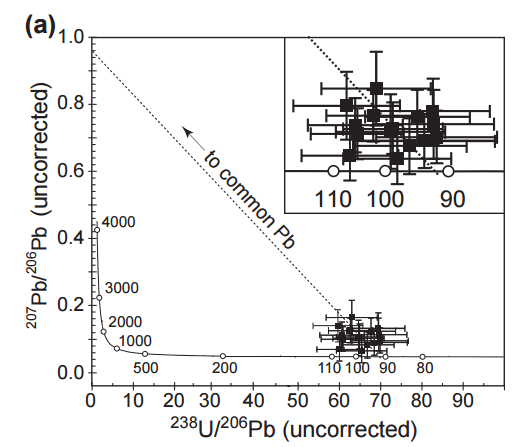
\includegraphics[width=0.5\textwidth]{1_a.png}
      	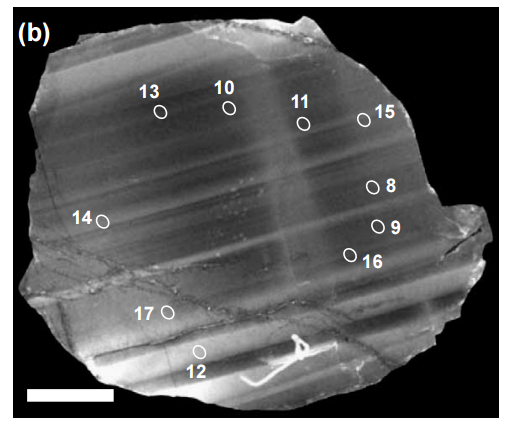
\includegraphics[width=0.5\textwidth]{1_b.png}
      	\caption{SHRIMP II U–Pb analyses of zircon standard KIM-5. (a)
      		Tera–Wasserburg concordia plot of 15 SHRIMP II analyses of two
      		different chips of KIM-5 made in two different sessions. Ages along
      		concordia are in Ma. Error bars are $2\sigma$. (b) CL image of one of the
      		KIM-5 chips used as an oxygen standard in this study (embedded in
      		mount 01JH36). Numbered analyses correlate to U–Pb analyses
      		8 through 17 listed in Appendix 2. Scale bar is 200 $\mu m$.}
\end{figure}
\bibliography{bibfile}
\end{document}


